% !TEX root = pfe-book2.tex
%!TEX TS-program = pdflatex
%!TEX encoding = UTF-8 Unicode


\cleardoublepage
%\mainmatter
\chapter{Temperature}
\label{ch-03}

\section{Thermometer}
If two differently heated bodies are brought into contact, the warmer one will cool off and the colder one will warm up. It is said that two such bodies exchange heat.

As we have already said, heat exchange is a kind of energy transfer; the body which gives off energy is said to be hotter. We feel that a body is hot if it makes our hand warm, transfers energy to it. On the contrary, if a body is felt to be cold, this means that it is taking energy away from our body.

Concerning a body which is giving off heat (i.e. giving off energy by means of heat exchange), we say: its temper­ature is higher than that of the body which is taking in this heat.

Observing whether an object of interest to us is cooling off or warming up in the presence of one or another body, we find ``its place'' in a row of heated bodies. Temperature is a kind of mark indicating for which bodies the object of interest to us will be a giver, and for which a receiver, of heat.

Temperature is measured by thermometers.

The structure of thermometers can be based on the utilization of various properties of bodies sensitive to temperature. The most frequently utilized property is the expansion of bodies during a rise in temperature.

If the body of a thermometer changes its volume when in contact with various bodies, this implies that these bodies have different temperatures. When the volume of the body of a thermometer is greater, the temperature is higher, and when the volume is smaller, the temperature is lower.

There are various substances that can serve as thermom­eters: liquids (such as mercury or alcohol), solids (such as metals), and gases. But different substances expand differently, and so mercurial, alcoholic, gaseous and other ``degrees'' will not coincide. Of course, two basic points, the melting point of ice and the boiling point of water, can always be marked on all thermometers. Therefore, all thermometers will indicate 0 and 100 degrees centi­grade identically. But bodies will not expand identically between 0 and 100 degrees. One body expands rapidly between 0 and 50 degrees on a mercury thermometer, and slowly in the second part of this interval, but another, vice versa.

Having made thermometers with differently expand­ing bodies, we will discover noticeable discrepancies in their readings, in spite of the fact that their readings will coincide for the basic points. Moreover, a water thermometer would lead us to the following discovery: if a body cooled to zero is placed on an electric stove, its ``water temperature'' would first fall and then rise. This happens because water at first decreases its volume when heated, and only later behaves ``normally'', i.e. increases its volume when heated.

We see that a rash choice of material for a thermometer can bring us to an impasse.

But then what should we be guided by in choosing a ``true'' thermometer? Which body would be ideal for this purpose?

We have already spoken about such ideal bodies. They are ideal gases. There are no interactions between the particles an ideal gas and studying the expansion of an ideal gas, we study how the motion of its molecules changes. This is precisely the reason why an ideal gas is an ideal body for a thermometer.

And it really is a striking fact that while water does not expand like alcohol (nor alcohol like glass, nor glass like iron), then hydrogen, oxygen, nitrogen and any other gas in a sufficiently rarefied state to deserve being called ideal expand in exactly the same fashion when heated.

Therefore, the changes in volume undergone by a def­inite amount of ideal gas serve as the basis for defining temperature in physics. Of course, in view of the fact that gases are highly compressible, one must be especially careful in seeing to it that the gas is under constant pres­sure.

In order to graduate a gas thermometer, we should accurately measure the volume of the gas we have chosen at \SI{0}{\celsius} and at \SI{100}{\celsius}. We shall divide the difference be­tween the volumes $V_{100}$ and $V_{0}$ into 100 equal parts. In other words, the change in the volume of the gas by $(V_{100} - V_{0})/100$ corresponds to one degree centigrade (\SI{1}{\celsius}).

Let us now suppose that our thermometer shows a volume $V$ What temperature $t\si{\celsius}$  corresponds to this volume? It is not difficult to comprehend that
\begin{equation*}%
t \si{\celsius} = \frac{V - V_{0}}{V_{100}-V_{0}} 100 \,\, \text{i.e.} \,\, \frac{t\si{\celsius}}{100} = \frac{V - V_{0}}{V_{100}-V_{0}}
\end{equation*}
By means of this equality, we assign each volume $V$ to a temperature $t$ and obtain the temperature scale\footnote{The centigrade scale at which \SI{0}{\celsius} is taken as the melting point of ice, and \SI{100}{\celsius} as the boiling point of water (both at the standard pressure of \SI{760}{\milli\meter\mercury}) is very convenient. In spite of this, the British and the Americans have so far been using a temperature scale which seems very strange to us. How, for example, will you react to the following sentence taken from an English novel: ``The summer wasn’t hot, the temperature was 60-70 degrees.'' A misprint? No, the Fahrenheit scale (\si{\fahrenheit}). The temperature in England rarely falls below \SI{-20}{\celsius}. Fahrenheit selected a mixture of ice and salt having approximately such a temperature and took this temperature for his zero. In the words of the inventor, the standard temperature of a human body was taken for 100 on this scale. However, in order to determine this point, Fahrenheit probably made use of the services of a slightly feverish person. On the \emph{Fahrenheit scale}, the average standard temperature of a human body is \SI{98}{\fahrenheit}. On this scale, water freezes at \SI{+32}{\fahrenheit} and boils at \SI{212}{\fahrenheit}. The conversion formula will be: 
$t \si{\celsius}= \dfrac{5}{9} (t - 32) \si{\fahrenheit}$.}
which physicists use.

With a rise in temperature, the volume of a gas increases without bound -- there is no theoretical limit to the growth in temperature. On the contrary, low (negative on the centigrade scale) temperatures have a limit.

What will happen when the temperature is lowered? A real gas will eventually turn into a liquid, and with an even greater fall in temperature, will solidify. The gas molecules will gather in a small volume. But what will this volume be equal to for a thermometer filled with an ideal gas? Its molecules do not interact with each other and do not have any volume of their own. Hence, a decrease in temperature brings an ideal gas to a zero vol­ume. It is quite possible to come as close as we wish in practice to a behaviour that is characteristic of an ideal gas, for example, to a zero volume. For this it is necessary to fill up the gas thermometer with more and more rare­fied gas. Therefore, we won’t go wrong by assuming the minimum volume of the gas equal to zero.

According to our formula, the lowest possible tempera­ture corresponds to a zero volume. This temperature is called the \emph{absolute zero} of temperature.

In order to determine the position of absolute zero on the centigrade scale, we must substitute zero for the vol­ume $(V = 0)$ in the temperature formula just derived. Consequently, the temperature of absolute zero is equal to $-100V_{0}/(V_{100}- V_{0})$.

It turns out that this remarkable point corresponds to a temperature of about $\SI{-273}{\celsius}$ (more precisely, $\SI{-273.15}{\celsius}$). 

Thus, there are no temperatures below absolute zero; for they would correspond to negative volumes of a gas. It doesn’t make sense to speak of lower temperatures. It is just as impossible to obtain temperatures below abso­lute zero as to make a wire with a diameter less than zero. It is impossible to cool a body at absolute zero, i.e. one cannot take energy away from it. In other words, bodies and the particles they are made of have the least possible energy at absolute zero. This implies that the kinetic energy equals zero and the potential energy as­sumes its least possible value at absolute zero.

Since absolute zero is the lowest temperature, it is only natural that the \emph{absolute scale} in which readings begin at absolute zero be used in physics, especially in those of its branches where low temperatures play an important role. It is clear that $T_{\text{abs}}  = (t + 273)\,\, \si{celsius}$. Room temperature will be about \SI{300}{\celsius} on the absolute scale. The absolute scale is also called the \emph{Kelvin scale}, in honour of the well-known 19th century English scien­tist, and the notation $T$ \si{kelvin} is employed in place of $T_{\text{abs}}$. A formula for a gas thermometer determining the abso­lute temperature $T$ can be written down in the form 
\begin{equation*}%
T = 100 \left(  \frac{V - V_{0}}{V_{100}-V_{0}} \right) + 273
\end{equation*}
Using the equality $100V_{0}/(V_{100}-V_{0}) = 273$, we arrive at the following simple result:
\begin{equation*}%
\frac{T}{273} = \frac{V}{V_{0}}
\end{equation*}
Therefore, the absolute temperature is simply proportion­al to the volume of an ideal gas.

Exact measurements of temperature require all kinds of contrivances on the part of the physicist. Mercury, al­cohol (for Arctic regions) and other thermometers are graduated by comparison with a gas thermometer over a rather wide temperature interval. However, it too is also unsuitable for temperatures very close to absolute zero (below \SI{0.7}{\kelvin}), when all gases liquefy, and also for temperatures above \SI{600}{\celsius}, when gases penetrate glass. Other principles of temperature measurement are used for high and very low temperatures.

As for practical methods of measuring temperature, they are manifold. Instruments based on electrical phenomena are of great significance. It is now important to remember only one thing -- during all measurements of temperature, we should be convinced that the reading obtained completely coincides with what a measurement of the expansion of a rarefied gas would give.

High temperatures arise in ovens, furnaces and burners. Temperatures of \SIrange{220}{280}{\celsius} are attained in baking ovens. Higher temperatures are applied in metallurgy -- hardening furnaces yield \SIrange{900}{1000}{\celsius}, forges yield \SIrange{1400}{1500}{\celsius}. Temperatures of \SI{2000}{\celsius} are attained in steel furnaces.

The records for high temperature in a furnace are ob­tained with the aid of electric arcs (about \SI{5000}{\celsius}). The arc flame makes it possible to deal with the most refractory metals.

And what is the temperature of the flame of a gas burn­er? The temperature in the inner bluish cone of flame is only \SI{300}{\celsius}. The temperature in the outer cone attains \SI{1800}{\celsius}.

Incomparably higher temperatures arise during the explosion of an atomic bomb. Judging by indirect esti­mates, the temperature at the centre of the explosion attains several million degrees.

Attempts have recently been made to obtain such ultrahigh temperatures in special laboratory installations built in the Soviet Union and in other countries. It has proved possible to attain temperatures up to several million degrees for very brief moments.

Ultrahigh temperatures also exist in nature, not on the Earth, but on other bodies in the Universe. In the centres of stars, the Sun in particular, the temperature attains tens of millions of degrees. But the surfaces of stars have a considerably lower temperature, not exceeding \SI{20000}{\celsius}. The surface of the Sun gets heated up to \SI{6000}{\celsius}.

\section{Ideal Gas Theory}
The properties of an ideal gas, giving us the definition of temperature, are very simple. The Boyle law is valid for constant temperatures: during changes in volume or pres­sure, the product $pV$ remains constant. For a constant pressure, the quotient $V/T$ is conserved, no matter how the volume or temperature changes. It is easy to unite these two laws. It is clear that the expression $pV/T$ re­mains the same as for a constant temperature but with changing $V$ and $p$; the same is true for a constant pressure but with changing $V$ and $T$. The expression $pV/T$ re­mains constant during a change not only in any pair, but also simultaneously in all three of the quantities $p$, $V$ and $T$. The law $pV/T = \text{const}$ is known as the \emph{equation of state of an ideal gas}.

An ideal gas is chosen for a thermometer because its properties depend only on the motion (but not on the interaction) of its molecules.

What is the nature of the relationship between the notion of molecules and temperature? To answer this ques­tion, it is necessary to find the relationship between the pressure of a gas and the motion of the molecules in it.

\begin{figure}[!ht]
\centering
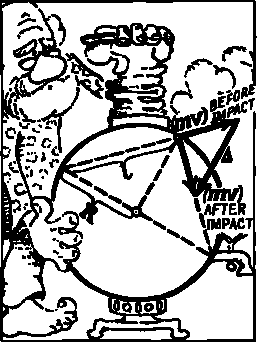
\includegraphics[width=0.4\textwidth]{figures/fig-03-01.pdf}
\caption{Finding pressure in a spherical vessel.}
\label{fig-3.1}
\end{figure}

In a spherical vessel of radius $R$, $N$ molecules of a gas are contained (\figr{fig-3.1}). Let us follow an arbitrary molecule, for example, one which is moving at a given moment from left to right along a chord of length $l$. We shall not pay attention to molecular collisions: such impacts do not affect the pressure. Having flown to the boundary of the vessel, the molecule will strike against the wall and fly off in some other direction with the same speed (the collision is elastic). Ideally, such a journey through the vessel might continue eternally. If $v$ is the molecular velocity, each impact will occur after $l/v$ seconds, i.e. each molecule will strike the wall $v/l$ times a second. The continual hail of impacts by the $N$ mole­cules unites into a single force of pressure.

According to Newton’s law, the force is equal to the change in momentum during a unit of time. Let us de­note the change in momentum at each impact by $\Delta$. This change occurs $v/l$ times a second. Consequently, the con­tribution to the force on the part of a single molecule will be $\Delta v/l$.

The momentum vectors before and after an impact, and also the momentum transfer $\Delta$ have been constructed in \figr{fig-3.1}. It follows from the similarity of the triangles arising in the construction that $\Delta/l = mv/R$. The con­tribution to the force on the part of a single molecule will take the following form:
\begin{equation*}%
\frac{mv^{2}}{R}
\end{equation*}
Since the length of the chord does not occur in the for­mula, it is clear that molecules moving along arbitrary chords make an identical contribution to the force. Of course, the change in momentum will be smaller for an oblique impact, but then the impacts in this case will be more frequent. Calculations show that these two effects exactly compensate for each other.

Since there are $N$ molecules in the sphere, the resultant force will be equal to
\begin{equation*}%
\frac{Nmv^{2}_{\textrm{av}}}{R}
\end{equation*}
where $v_{\textrm{av}}$ is the average molecular velocity.

The pressure $p$ of the gas equal to the force divided by
the surface area of the sphere, $4\pi R^{2}$, is
\begin{align*}%
p &= \frac{Nmv^{2}_{\textrm{av}}}{4 \pi R^{2}R} = \frac{\frac{1}{3}Nmv^{2}_{\textrm{av}}}{\frac{4}{3}\pi R^{2}} \\
& = \frac{Nmv^{2}_{\textrm{av}}}{3V}
\end{align*}
where $V$ is the volume of the sphere. 

Therefore,
\begin{equation*}%
pV = \frac{1}{3} Nmv^{2}_{\textrm{av}}
\end{equation*}
This equation was first derived by Daniel Bernoulli in 1738.\footnote{Of Swiss origin, D. Bernoulli worked and lived in Russia; he was a member of the St. Petersburg Academy of Sciences. No less well known is the activity of Johann (Jean) Bernoulli and Jakob (Jacques) Bernoulli. All three were brothers, not namesakes.}

It follows from the equation of state of an ideal gas that $pV = \textrm{const} \cdot T$; we see from the equation just derived that $pV$ is proportional to $v^{2}_{\textrm{av}}$. Hence,
\begin{equation*}%
T \propto v^{2}_{\textrm{av}} \,\, \text{or} \,\,  v_{\textrm{av}} \propto \sqrt{T}
\end{equation*}
i.e. the average velocity of an ideal gas molecule is proportional to the square root of the absolute temperature.

\section{Avogadro's Law}

Assume that a substance is a mixture of different mole­cules. Isn’t there a physical quantity characterizing a motion which would be identical for all these molecules, say, for hydrogen and oxygen, provided their tempera­tures are identical?

Mechanics yields an answer to this question. It can be proved that the average kinetic energy $mv^{2}_{\textrm{av}}/2$ of the trans­lator motion will be identical for all molecules.

This implies that for a given temperature, the average square of the molecular velocities is inversely proportion­al to the mass of the particles:
\begin{equation*}%
v^{2}_{\textrm{av}} \propto \frac{1}{m} \,\, \text{or} \,\, v_{\textrm{av}} \propto \frac{1}{\sqrt{m}} 
\end{equation*}
Let us return to the equation $pV = (1/3) Nmv^{2}_{\textrm{av}}$. Since the quantities $mv^{2}_{\textrm{av}}$ are identical for all gases at a given temperature, the number $N$ of molecules contained in a given volume $V$ at a definite pressure $p$ and temperature $T$ is identical for all gases. This remarkable law was first formulated by Amedeo Avogadro (1776-1856).

But how many molecules are there in \SI{1}{\centi\meter\cubed}? It turns out that there are \num{2.7d19} molecules in \SI{1}{\centi\meter\cubed} at \SI{0}{\celsius} and \SI{760}{\milli\meter\mercury}. This is an enormous number. So that you can feel just how great it is, let us give an example. Suppose that gas is flowing out of a \SI{1}{\centi\meter\cubed} vessel with such a speed that a million molecules leave each second. It isn’t hard to calculate that it will take the vessel a million years to get rid of the gas!

Avogadro’s law shows that under a definite pressure and temperature, the ratio of the number of molecules to the volume in which they are contained, $N/V$, is a quan­tity that is identical for all gases.

Since the density of a gas $p = Nm/V$, the ratio of the densities of gases is equal to that of their molecular masses:
\begin{equation*}%
\frac{\rho_{1}}{\rho_{2}} = \frac{m_{1}}{m_{2}}
\end{equation*}
The relative masses of molecules can therefore be determined by simply weighing gaseous substances. Such measurements once played a great role in the development of chemistry. It also follows from Avogadro’s law that for a mole of any substance in the state of an ideal gas, $pV = kN_{A}T$, where $k$ is a universal constant (named after the famous German physicist Ludwig Boltzmann) equal to \SI{1.38d-16}{\erg\kelvin}. The product $R = kN_{A}$ is called the universal gas constant.

The ideal gas law is often written as
\begin{equation*}%
pV = \mu RT
\end{equation*}
where $\mu$ is the amount of substance expressed in moles.

This equation is frequently applied in practice.

\section{Molecular Velocities}

Theory shows that for a constant temperature, the aver­age kinetic energy of molecules, $mv^{2}_{\textrm{av}}/2$, is identical. Ac­cording to our definition of temperature, this average kinetic energy of the translatory motion of the molecules of a gas is proportional to the absolute temperature.

Combining the ideal gas equation with Bernoulli’s equation we obtain 
\begin{equation*}%
\left( \frac{mv^{2}}{2} \right)_{\textrm{av}} = \frac{2}{3} kT
\end{equation*}
Temperature measurements with a thermometer filled with an ideal gas add a meaning of rare simplicity to this measure. The temperature is proportional to the average value of the energy of translatory motion of the mole­cules. Since we live in three-dimensional space, we can say that a point moving at random has three degrees of freedom. Consequently, there is $kT/2$ energy per degree of freedom of a moving particle.

Let us determine the average speed of oxygen mole­cules at room temperature, which we take to be $\SI{27}{\celsius} = \SI{300}{\kelvin}$ in round numbers. The molecular mass of oxygen is 32, so the mass of one molecule equals $32/(\num{6d23})\si{\gram}$. A simple computation yields $v_{\textrm{av}} = \SI{4.8d4}{\centi\meter\per\second}$, i.e. about \SI{500}{\meter\per\second}. Molecules of hydrogen move considerably faster. Their masses are 16 times as small, and their speeds are $\sqrt{16} = 4$ times as great, i.e. are about 2 km/s at room temperature. Let us estimate the thermal speed of a small particle which is visible through a microscope. An ordinary microscope permits us to see a dust particle of \SI{1}{\micro\meter} (\SI{d-4}{\centi\meter}) in diameter. The mass of such a particle with a density close to unity will be in the neighbourhood of \SI{5d-13}{\gram}. We obtain about  \SI{0.5}{\centi\meter\per\second} for its speed. It is not surprising that such motion is quite noticeable.

The speed of the Brownian movement of a particle with a mass of \SI{0.1}{\gram} will be only \SI{d-6}{\centi\meter\per\second} in all. It is no wonder that we do not see the Brownian movement of such particles.

We have spoken of the average speed of a molecule. But not all molecules move with the same speed; a certain fraction of the molecules move faster, but others move slower. It turns out that this can all be calculated. We shall only present the results.

At a temperature of about \SI{15}{\celsius}, for example, the average speed of nitrogen molecules is equal to \SI{500}{\meter\per\second}; 59\% of the molecules move with speeds between 300 and \SI{700}{\meter\per\second}. Only 0.6\% of the molecules move with small speeds -- from 0 to \SI{100}{\meter\per\second}. There are only 5.4\% of fast molecules with speeds greater than \SI{1000}{\meter\per\second} (\figr{fig-3.2}).

\begin{figure}[!ht]
\centering
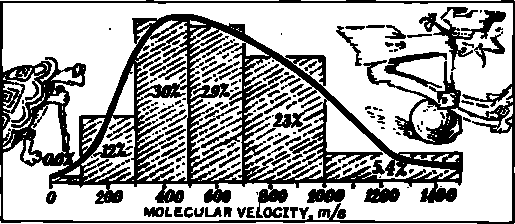
\includegraphics[width=\textwidth]{figures/fig-03-02.pdf}
\caption{A graph showing the distribution of velocities in a gas.}
\label{fig-3.2}
\end{figure}

Each column is constructed with its base covering the velocity range it refers to and the area of each column is proportional to the percentage of molecules whose veloc­ity lies within this range.

It is also possible to calculate the distribution of molecules over the energy of their translatory motion.

The number of molecules whose energy is more than double the average is less than 10\%. The fraction of still more “energetic” molecules falls off faster and faster as the energy increases. Thus, the number of molecules whose energy is at least four times as large as the average is only 0.7\%, eight times as large as the average $0.06 \times
 \num{d-4}$\%, 16 times as large as the average $2 \times \num{d-8}$\%. 
 
The energy of an oxygen molecule moving with a speed of \SI{11}{\kilo\meter\per\second} is equal to \SI{32d-12}{\erg}. The average energy of a molecule at room temperature is equal to only \SI{6d-14}{\erg}. Therefore, the energy of an ``eleven-kilo­ metre molecule'' is at least 500 times as great as the ener­gy of a molecule with the average speed. It is not surpris­ing that the fraction of the molecules with speeds higher than \SI{11}{\kilo\meter\per\second} is equal to an unimaginably small number -- of the order of \num{d-300}.

But why are we intrigued with the speed of \SI{11}{\kilo\meter\per\second}? In the first book we spoke of the fact that only bodies having this speed can escape from the Earth. Hence, molecules which have risen to a great height can lose their ties to the Earth and take off in a distant interplane­tary trip, but for this it is necessary to have a speed of \SI{11}{\kilo\meter\per\second}. The fraction of such fast molecules, as we have seen, is so negligible that there is no danger of the Earth’s losing its atmosphere even in the course of a thousand million years.

The rate of leaving the atmosphere depends to an ex­traordinarily great degree on the gravitational energy $GMm/r$. If the average kinetic energy of a molecule is many times less than the gravitational energy, the escape of the molecules from the Earth is practically impos­sible. The gravitational energy on the surface of the Moon is 20 times as small, which gives an oxygen molecule a ``runaway'' energy of \SI{1.5d-12}{\erg}. This value exceeds that of the average kinetic energy of a molecule by a factor of only 20-25. The fraction of the molecules capable of breaking away from the Moon is equal to \num{d-17}. This is already entirely different than \num{d-300}, and computations show that the air would leave the Moon quickly enough for interplanetary space. It is not surprising that there is no atmosphere on the Moon.


\section{Thermal Expansion}

If a body is heated, the motion of its atoms (molecules) will be more intensive. They will start pushing each other away and will occupy more space. The following well-known fact is explained by this: solids, liquids and gases expand when heated.

We don’t have to say much about the thermal expansion of gases: in fact, the proportionality of gas temperature to volume was made the basis of our temperature scale.
We see from the formula $V = V_{0}T/273$ that the volume of a gas under a constant pressure grows by 1/273 (i.e. by 0.0037) of its value at \SI{0}{\celsius} for each \SI{1}{\celsius} increase in tem­perature (this situation is sometimes called Gay-Lussac’s law).

Under ordinary conditions, i.e. at room temperature and standard atmospheric pressure, most liquids expand one-third to one-half as much as gases.

We have already spoken more than once of the anoma­lous expansion of water. The volume of water decreases as it is heated up from 0 to \SI{4}{\celsius}. This anomaly in the expansion of water plays a colossal role in organic life on the Earth. In autumn, the upper layers of water become denser and sink to the bottom as they cool off. Warmer water, rising from below, takes their place. But such a mixing takes place only until the temperature of the water falls to \SI{4}{\celsius}. With a further fall in temperature, the upper layers will no longer contract, will therefore not become heavier and will not sink to the bottom. Starting with this temperature, the upper layer, gradually cooling off, reaches zero degrees and freezes.

It is only this peculiarity of water that prevents rivers from freezing down to their beds. If water were to sud­denly lose its remarkable anomaly, the disastrous con­sequences of this can be easily pictured even by a person without a rich imagination.


The thermal expansion of solids is considerably less than that of liquids. It is hundreds and thousands of times less than the expansion of gases.

Thermal expansion is an annoying hindrance in many cases. Thus, a change in the sizes of the moving parts of a clockwork with a change in temperature would lead to a change in the speed of the clock, if a special alloy, in­ var (invariant means unchanging, whence the name ``invar''), were not used for these delicate components. Invar, steel with a large nickel content, is widely used in the instrument manufacture. An invar rod is lengthened by only one-millionth when its temperature increases by \SI{1}{\celsius}.

An apparently negligible thermal expansion of a solid body can lead to serious consequences. The reason for this is that the low compressibility of solids makes it hard to hinder their thermal expansion.

When heated by \SI{1}{\celsius}, a steel rod will increase in length by only one-hundred-thousandth, i.e. by an amount unnoticeable to the unaided eye. However, in order to prevent the expansion and compress the rod one-hundred-thousandth, a force of \SI{20}{\kgf} on \SI{1}{\centi\meter\squared} is needed. And this is merely for cancelling the effect of a rise in temperature by only \SI{1}{\celsius}.

The forces arising from thermal expansion can lead to breakages and catastrophes if they are not reckoned with. Thus, in order to avoid the action of these forces, the rails of a railroad-bed are laid with clearances. One has to remember these forces when handling glassware which is easily cracked by non-uniform heating. It is therefore the practice in laboratories to use vessels made of quartz glass (fused quartz, silicon dioxide, exists in an amorphous state), which lack this drawback. For one and the same rise in temperature, a copper bar will be lengthened by a millimetre, while the same sized bar of quartz glass will change its length by the unnoticeable amount of 30-40 \si{\micro\meter}. The expansion of quartz is so insignificant that a quartz vessel can be heated by several hundred degrees and then thrown into water without any fear.

\section{Heat Capacity}

The internal energy of a body also depends, of course, on its temperature. The more a body must be heated, the greater is the energy required. In order to raise the tem­perature of a body from $T_{1}$ to $T_{2}$, it is required to supply an energy
\begin{equation*}%
Q=C(T_{2}-T_{1})
\end{equation*}
to it in the form of heat. Here $C$ is the proportionality factor, which is called the \emph{heat capacity} of the body. The definition of the concept of heat capacity follows from the formula: $C$ is the amount of heat necessary for raising the temperature by \SI{1}{\celsius}. The heat capacity also derends on the temperature: rises in temperature from 0 to \SI{1}{\celsius} and from 100 to \SI{101}{\celsius} require somewhat different amounts of heat.

The quantity $C$ is usually referred to a unit mass and called the \emph{specific heat}. It is then denoted by the small letter $c$.

The amount of heat which goes to heat up a body of mass m is given by the following formula:
\begin{equation*}%
Q = mc (T_{2} — T_{1})
\end{equation*}
In what follows we shall make use of the concept of specific heat capacity, but shall speak of the heat capac­ity of a body for the sake of conciseness. An additional guide will always be the dimension of the quantity.

The value of heat capacity varies within a rather wide range. Of course, the heat capacity of water in calorie per degree is equal to unity by definition.

Most bodies have a heat capacity less than that of water. Thus, most oils, alcohols and other liquids have heat capacities close to \SI{0.5}{\calorie\per\gram\per\kelvin}. Quartz, glass and sand have a heat capacity of the order of \SI{0.2}{\calorie\per\gram\per\kelvin}. The heat capacity of iron and copper is about \SI{0.1}{\calorie\per\gram\per\kelvin}. And here are examples of the heat capacities of some gases: hydrogen, \SI{3.4}{\calorie\per\gram\per\kelvin}; air, \SI{0.24}{\calorie\per\gram\per\kelvin}.

The heat capacities of all bodies decrease, as a rule, with a fall in temperature, and assume negligible values for most bodies at temperatures close to absolute zero. Thus, the heat capacity of copper is equal to only 0.0035 at \SI{20}{\kelvin}; this is twenty-four times less than at room tem­perature.

A knowledge of heat capacities may prove useful for solving various problems on the distribution of heat among bodies.

The difference between the heat capacities of water and soil is one of the causes determining the distinction between maritime and continental climates. Possessing approximately five times as great a heat capacity as soil, water warms up slowly and cools off just as slowly.

In summer in maritime regions, the water, having warmed up more slowly than the land, cools the air, but in winter, the warm sea gradually cools off, yielding heat to the air and making the frost less severe. It is not diffi­cult to calculate that \SI{1}{\meter\cubed} of sea water, cooling off by \SI{1}{\celsius}, warms up \SI{3000}{\meter\cubed} of air by \SI{1}{\celsius}. Consequently, in maritime regions the variations in temperature and the difference between winter and summer temperatures are less substantial than in continental regions.

\section{Thermal Conductivity}
Each object can serve as a ``bridge'' along which heat passes from a warmer body to a cooler one. For example, a tea spoon placed in a glass of hot tea is such a bridge.

Metallic objects conduct heat very well. The top of the spoon placed in the glass will become warm in the course of a second.

If it is necessary to stir a hot mixture, the handle of the stirrer must be made of wood or plastic. These solids conduct heat a thousand times worse than metals. We say ``conduct heat'', but could just as well have said ``con­duct cold''. Of course, the properties of a body do not change as a result of the direction in which a heat flow is passing through it. In freezing weather we are careful not to touch metals with our bare hands outdoors, but grasp wooden handles without fear.

Among the poor heat conductors, they are also called heat insulators, are wood, brick, glass and plastic. The walls of houses, ovens and refrigerators are made of these materials.

Among the good conductors are all the metals. The best conductors are copper and silver -- they conduct heat twice as well as iron.

Of course, not only solids can serve as ``bridges'' for the transfer of heat. Liquids also conduct heat, but much worse than metals. The thermal conductivity of metals is hundreds of times greater than that of solid and liquid non-metallic bodies.

In order to demonstrate the poor thermal conductiv­ity of water, the following experiment is performed. A piece of ice is fastened to the bottom of a test-tube filled with water, while the top of the test-tube is heated over a gas burner; the water begins boiling, but the ice is still not melting. If the test-tube were without water and made of metal, then the piece of ice would begin melting almost immediately. Water conducts heat about two hundred times worse than copper.

Gases conduct heat tens of times worse than condensed non-metallic bodies. The thermal conductivity of air is twenty thousand times smaller than that of copper.

The poor thermal conductivity of gases permits us to hold in our hands a piece of dry ice whose temperature is \SI{-78}{\celsius}, and to even hold on our palms a drop of liquid nitrogen having a temperature of \SI{-196}{\celsius}. If we do not squeeze these cold objects with our fingers, there will be no ``bum''. The reason consists in the fact that when the drop of liquid or the piece of solid is boiling very energet­ically, it is covered by a ``vapour jacket'', and the layer of gas so formed serves as a heat insulator.

The spheroidal state of a liquid, this is what one calls the state in which drops are covered by vapour, is formed whenever water gets into a very hot frying-pan.\footnote{This is the so called Leidenfrost effect. -- Damitr} Drops of boiling water, having fallen on one’s palm, severely burn one’s hand, although the difference in temperature between boiling water and a human body is less than that between a hand and liquid air. Since one’s hand is colder than the drops of boiling water, heat leaves the drops, the boiling ceases and no vapour jacket is formed.

It isn’t hard to understand that the best heat insulator is a vacuum -- emptiness. There are no carriers of heat in a vacuum, and so the thermal conductivity will be at a minimum.

Therefore, if we want to create a thermal shield, hide something warm from something cold or vice versa, the best thing to do is to erect a casing with double walls and pump the air out of the space between them. When doing this, we come across the following curious phenomenon. If we keep track of the change in thermal conductivity of the gas as it is being rarefied, we shall observe that right until the moment when the pressure reaches sev­eral millimetres of mercury column the thermal conduc­tivity remains practically constant. Our expectations are only justified when, with the passage to a higher vacuum, the thermal conductivity sharply falls off.

But what is the cause of this?

In order to understand this phenomenon, we must try to visualize the process of heat transfer in a gas.

Heat transfer from a warm place to a cold one takes place by means of the transmission of energy from one molecule to a neighbouring one. It is clear that collisions between fast and slow molecules usually lead to an ac­celeration of the slow molecules and a deceleration of the fast ones. And this means that the hot place will become colder, while the cold place will warm up.

But how will a decrease in pressure affect heat transfer? Since a decrease in pressure lowers the density, the num­ber of collisions between fast and slow molecules, during
which a transmission of energy occurs, will also decrease. This would decrease the thermal conductivity. However, a decrease in pressure leads, on the other hand, to an increase in the mean free path of the molecules, which therefore transfer heat by greater distances, and this tends to increase the thermal conductivity. Computations show that these effects compensate for each other, and so the ability to transfer heat does not change for some time as the air is being pumped out.

This will be the case until the vacuum becomes so con­siderable that the mean free path is comparable to the distance between the walls of the vessel. Now a further decrease in the pressure can no longer change the mean free path of the molecules, which are ``hopping around'' from wall to wall: the fall in density is not compensated for, and so the thermal conductivity rapidly falls in proportion to the pressure, reaching negligible values as a high vacuum is attained. The construction of a vacuum bottle is based on the use of the properties of a vacuum. Vacuum bottles are very widespread: they are applied not only for the conservation of hot and cold foods but also in science and technology. In such a case they are called Dewar flasks (vessels), in honour of their inventor. Liq­uid air, nitrogen and oxygen are transported in such vessels. Later we shall tell how these gases are obtained in a liquid state.\footnote{Everyone who has seen cylinders of vacuum bottles noticed that their walls are always silver-plated. But why? The fact is that thermal conductivity is not the only means of trans­ferring heat. There exists yet another way to transfer heat, which we shall speak of in another book, so-called radiation. Under ordinary conditions, it is much weaker than thermal conductivity, but is nevertheless quite noticeable. The walls of vacuum bottles are covered with a coating of silver precisely in order to weaken the radiation.}

\section{Convection}

But if water is such a poor heat conductor, how does it warm up in a tea-kettle? Air conducts heat even worse; then it isn’t clear why the same temperature is established in all parts of a room.

Water in a tea-kettle quickly boils because of gravity. The lower layers of water, having warmed up, expand, become lighter and rise to the top, with cold water tak­ing their place. A rapid heating occurs thanks only to \emph{convection} (derived from the Latin \emph{convectus} meaning ``bring together''). It wouldn’t be so easy to heat up water in a tea-kettle located in an interplanetary rocket.

Somewhat earlier explaining why rivers do not freeze down to the bottom, we spoke of another case of convec­tion currents of water without using this word.

Why are the radiators of a central heating placed near the floor? Why is the ventilation window made in the upper part of a window? It might be more convenient to open a ventilation window if it were lower down, and it might not be a bad idea to place radiators under the ceiling, so that they did not get in the way. If we were to follow such advice, we would soon discover that the room is not being warmed up by the radia­tor and not being aired when the ventilation window is open.

The same thing takes place with the air in a room as with the water in a tea-kettle. When the radiator is turned on, the air in the lower layers of the room begins warm­ ing up. It expands, becomes lighter and rises towards the ceiling. Heavier layers of cold air arrive in its place. And they, having warmed up, leave for the ceiling. A contin­uous air current thus arises in the room, with warm air moving up from below and cold air moving down from above. Opening a ventilation window in winter, we admit a stream of cold air into the room. It is heavier than the air in the room, and so goes down, forcing out the warm air, which rises towards the top of the room and leaves through the ventilation window.

A kerosene lamp flames up well only when it is covered with a tall piece of glass. One should not think that the glass is needed only in order to shield the flame from the wind. Even in the calmest weather, the brightness of the flame immediately increases when the glass is put on the lamp. The role of the glass consists in intensifying the stream of air approaching the flame -- in creating a draught. This occurs because the air inside the glass, deprived of the oxygen that was used for the burning, quick­ly warms up and rises, while pure cold air moves into its place through the holes made in the burner of the lamp.
The taller the glass, the better will the lamp burn. In fact, the speed with which cold air rushes into the burner of the lamp depends on the difference in weight between the heated column of air in the lamp and the cold air outside it. The higher the column of air, the greater this difference in weight, and so the faster the movement.

Factory chimneys are also made high for this reason. An especially rapid influx of air, a good draught, is needed for a factory furnace. It is achieved as a result of a high chimney.

The lack of convection in a rocket devoid of weight makes it impossible to use matches, lamps or gas burners: the products of combustion would smother the flame. Air is a poor conductor; we can conserve heat with its aid, but only under one condition: if we avoid convection, the mixing of warm and cold air, which will bring to naught the thermal-insulation properties of air.


The elimination of convection is achieved by applying various kinds of porous and fibrous bodies. It is difficult for air to move inside such bodies. All bodies of this kind are good heat insulators, thanks only to their ability to retain a layer of air. But the thermal conductivity of the substance itself of which the fibres or the walls of the
pores consist can be not very small.

A good fur coat is made of a dense fur containing as many fibres as possible; eiderdown can be used to make warm sleeping bags weighing less than half a kilogram, due to the exceptional thinness of its fibres. Half a kilo­gram of this down can ``detain'' as much air as tens of kilograms of sheet wadding.

Storm windows are made in order to reduce the con­vection. The air between the panes does not participate in the mixing of layers of air which takes place within the room.

On the contrary, every movement of the air intensifies the mixing and increases the transfer of heat. This is precisely why we fan ourselves or turn on the ventilator when we want the heat to go away faster. This is also what makes it colder in the wind. But if the air temperature is higher than one’s body temperature, the mixing has the opposite effect, and a wind feels like a hot breath of air.

The problem involved in a steam boiler consists in obtaining steam heated to the required temperature as quickly as possible. The natural convection in a gravita­tional field is quite insufficient for this. Therefore, the creation of an intensive circulation of water and steam, leading to the mixing of warm and cold layers, is one of the basic problems in the construction of steam boilers.
